% !TeX encoding = UTF-8
% !TeX spellcheck = en_US
% !TeX root = ../MasterThesis_OlivierChurlaud_2016.tex

\chapter{Basics of particle accelerator physics}
\label{sec:acc_physics}
In order to be able to localize and correct perturbation, the effects of a perturbation on a particle trajectory must be clearly understood. This section will the particle motion in circular accelerator and define the parameters needed for the following explanations.

The beam trajectory can be studied in various ways. One easier and well used method stems from the field of linear beam optics (by analogy between beam and light focusing and steering). Here will be solely described what is needed in the next sections. A full reference can be found in~\cite{book:wille}. This section is mostly inspired by the chapter 3 of this same reference.

\section{Geometry -- Frame of reference -- Kinematics}
The term \emph{orbit} refers to the ideal trajectory of the particles, which is fixed by the construction of the accelerator.

The frame of reference is $K=(\vec{e}_x,\vec{e}_y, \vec{e}_s)$, which origin follows the beam. $\vec{e}_x$ is the horizontal axis directed towards the exterior of the orbit and normal to its curve, $\vec{e}_y$ is the vertical axis and $\vec{e}_s$ the tangential axis to the orbit.
\begin{figure}
    \centering
    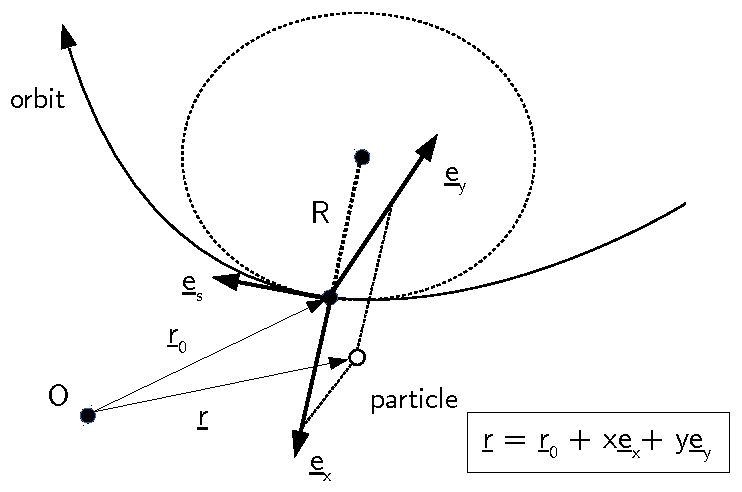
\includegraphics[width=0.8\linewidth]{img/orbit_coordinates.pdf}
    \caption[Description of the co-moving coordinate system]{\label{fig:coordinate system}Description of the co-moving coordinate system (inspired by~\cite{book:wille}, Fig~3.2)}
\end{figure}
Let $\varphi$ be the azimuth angle, oriented by $\vec{e}_y$. Then, since $ds = -R d\varphi$, it can be written
\begin{equation}
\frac{d \varphi}{d t}  = -\frac{1}{R} \frac{d s}{d t}.
\end{equation}

Using the derivation formula of polar coordinate yields
\begin{align}
&\dot{\vec{e}}_x = \frac{d\vec{e}_x}{d t} = -\dot{\varphi} \vec{e}_s = \frac{1}{R} \dot{s}\vec{e}_s \nonumber \\
&\dot{\vec{e}}_y = 0 \\
&\dot{\vec{e}}_s = \frac{d\vec{e}_s}{d t} = \dot{\varphi} \vec{e}_x = -\frac{1}{R} \dot{s}\vec{e}_x \nonumber.
\end{align}

Let $\vec{r} = \vec{r}_0 + x\vec{e}_x + y \vec{e}_y$ be the position of a given particle in a Galilean reference frame (with $\vec{r}_0$ the position of the origin of the moving coordinates, see \cref{fig:coordinate system}) and let $x'$ be the spatial derivative with respect to $s$ so that:
\begin{equation}
\begin{aligned}
&\dot{x}= \frac{dx}{ds}\frac{ds}{dt} = x'\dot{s}  \\
&\ddot{x}= x''\dot{s}^2+x'\ddot{s}.
\end{aligned}
\end{equation}
It follows, after some algebraic manipulations:
\begin{align}
\label{eq:kinematics}
&\vec{r} = \vec{r}_0 + x\vec{e}_x + y \vec{e}_y \nonumber \\
&\dot{\vec{r}}= x' \dot{s} \vec{e}_x + y'\dot{s} \vec{e}_y  + \left(1+\frac{x}{R}\right)\dot{s}\vec{e}_s\\
&\ddot{\vec{r}}= \left[x'' \dot{s}^2 + x' \ddot{s} - \left( 1+\frac{x}{R} \right)\frac{\dot{s}^2}{R}\right] \vec{e}_x + (y''\dot{s}^2 + y'\ddot{s}) \vec{e}_y \nonumber \\
& \hspace{14em} + \left[\frac{2}{R}x'\dot{s}^2 +\left(1+\frac{x}{R}\right)\ddot{s}\right]\vec{e}_s \nonumber
\end{align}

\section{Assumptions}
The following assumptions are assumed to be valid.
\begin{description}
    \item{A1 --} The particles move essentially parallel to $\vec{e}_s$: in the first order
    \begin{equation*}
        \vec{v} = v_s \vec{e}_s.
    \end{equation*}
    \item{A2 --} The magnetic field has only transverse components:
        \begin{equation*}
        \vec{B} = (B_x, B_y, 0).
        \end{equation*}
    \item{A3 --} The electric field is negligible with respect to the magnetic field.
    \item{A4 --} The velocity of the particle varies very slowly in a magnet: $\ddot{s} \approx 0$.
    \item{A5 --} The particles move at relativistic velocities, so the effect of the magnetic field is negligible on longitudinal components: only transverse components will be considered.
    \item{A6 --} The momentum of the particles is $p = p_0+\Delta p$, with the condition $\Delta p \ll p_0$ (which is well satisfied in accelerators).
\end{description}

\section{Equation of motion}
\label{sec:eq_motion}
Newton's second law can be applied with the Lorentz force
\begin{equation}
\dot{\vec{p}} = e(\vec{E}+\vec{v} \times \vec{B})
\end{equation}
which according to (A3) becomes
\begin{equation}
\ddot{\vec{r}} = \frac{e}{m}(\dot{\vec{r}} \times \vec{B})
\end{equation}

According to (A2), the magnetic field is only transversal, which yields
\begin{equation}
\label{eq:lorentz_transv}
\ddot{\vec{r}} = \frac{e}{m}(\dot{\vec{r}} \times \vec{B})
= \frac{e}{m}
    \begin{pmatrix}
        -\left(1+\frac{x}{R}\right)\dot{s}B_y \\
        \left(1+\frac{x}{R}\right)\dot{s}B_x \\
        x'\dot{s}B_y - y'\dot{s}B_x
    \end{pmatrix}.
\end{equation}

Using (A5), the $s$-component does not need to be considered and using (A4) in \cref{eq:kinematics} allows to remove every $\ddot{s}$ factors, so that \cref{eq:lorentz_transv} can be rewritten as
\begin{equation}
\begin{aligned}
x'' \dot{s}^2 - \left(1+\frac{x}{R}\right)\frac{\dot{s}^2}{R}
&= -\frac{e}{m} \left(1+\frac{x}{R}\right)\dot{s}B_y \\
y'' \dot{s}^2 &=    \left(1+\frac{x}{R}\right)\dot{s}B_x.
\end{aligned}
\end{equation}
Finally, because $p=mv$ and using \cref{eq:kinematics} combined with (A1),
\begin{equation}
m = \frac{p}{v} = \frac{p}{\scal{\vec{v}}{\vec{e}_s}} = \frac{p}{\left(1+\frac{x}{R}\right)\dot{s}}
\end{equation}
can be substituted to obtain
\begin{equation}
\begin{aligned}
x''-\left(1+\frac{x}{R}\right)\frac{1}{R} &= -\frac{e}{p} B_y\left(1+\frac{x}{R}\right)^2 \\
y'' &= \frac{e}{p} B_x\left(1+\frac{x}{R}\right)^2
\end{aligned}
\end{equation}

According to (A6), it can be written to first order
\begin{equation*}
\frac{1}{p} = \frac{1}{p_0} \left(1-\frac{\Delta p}{p_0}\right).
\end{equation*}

Furthermore the magnetic field can be approximated to first order with:
\begin{equation}
\frac{e}{p_0} B_y = \frac{1}{R}-kx \qquad\qquad \frac{e}{p_0} B_x = -ky
\end{equation}
which yields
\begin{equation}
\begin{aligned}
x''-\left(1+\frac{x}{R}\right)\frac{1}{R} &= -\left(\frac{1}{R}-kx\right)\left(1-\frac{\Delta p}{p_0}\right)\left(1+\frac{x}{R}\right)^2 \\
y'' &= -ky\left(1-\frac{\Delta p}{p_0}\right)\left(1+\frac{x}{R}\right)^2
\end{aligned}
\end{equation}

Finally removing terms of second order ($\frac{x}{R} \ll 1$, $\frac{\Delta p}{p_0} \ll 1$) leads to the linear equations of motion in a magnetic structure:

\begin{empheq}[box=\fbox]{equation}
\label{eq:motion_particle}
\begin{aligned}
x''(s) + \left(\frac{1}{R^2(s)} - k(s)\right) x(s) &= \frac{1}{R(s)}\frac{\Delta p}{p_0} \\
y''(s) + k(s) y(s) &= 0
\end{aligned}
\end{empheq}

\section{Beta function and betatron oscillation}
\label{sec:beta_func}
The beta function will provide a description of properties of a beam of many particles.

The only further assumption is that $\frac{1}{R} = 0$ and $\frac{\Delta p}{p_0}=0$. The orbit curve is thus assumed almost flat and the momentum deviation negligible. \Cref{eq:motion_particle} turns in Hill's differential equation:
\begin{equation}
\label{eq:hill_diff}
	x''(s) - k(s) x(s) = 0
\end{equation}
which solution is the transverse oscillation of the orbit, or \emph{betatron oscillation}
\begin{equation}
\label{eq:hill_sol_cst}
x(s) = A u(s) \cos \left(\Psi(s)+\phi \right).
\end{equation}

The phase and the amplitude depend of the position $s$; $A$ and $\phi$ being integration constants.

Inserting \cref{eq:hill_sol_cst} in \eqref{eq:hill_diff} it follows
\begin{equation}
A\left[u''- u \Psi'^2 - k u \right] \cos\left(\Psi+\phi\right) - A\left[2u'\Psi'+u\Psi''\right]\sin\left(\Psi+\phi\right) = 0.
\end{equation}

$A \ne 0$ and $\Psi(s)$ having different values for every $s$, the previous equation provides two conditions
\begin{align}
u''- u \Psi'^2 - k u = 0 \label{eq:hill_cond1}\\
2u'\Psi'+u\Psi'' = 0 \label{eq:hill_cond2}.
\end{align}

\Cref{eq:hill_cond2} leads to
\begin{equation}
2\frac{u'}{u} + \frac{\Psi''}{\Psi'} = 0
\end{equation}
which can be integrated as
\begin{equation}
\label{eq:phase_psi}
\Psi(s) = \int \limits_{0}^{s} \frac{d\sigma}{u^2(\sigma)}.
\end{equation}

The \emph{beta function} $\beta(s)$ is defined as
\begin{equation}
\label{eq:beta_func}
\beta(s) := u^2(s).
\end{equation}
and allows to rewrite
Substituting $A = \sqrt{\varepsilon}$ provides the final trajectory equation
\begin{empheq}[box=\fbox]{equation}
	\label{eq:orbit_equation}
	x(s) = \sqrt{\varepsilon \beta(s)} \cos\left(\Psi(s)+\phi \right)
\end{empheq}

The constant $\varepsilon$ is termed \emph{emittance} and the envelop of the orbit at each position $s$ is $E(s) = \sqrt{\varepsilon \beta(s)}$, which defines the size of the beam.

Finally, deriving $x(s)$ leads to
\begin{align}
    x'(s) &= \frac{\sqrt{\varepsilon \beta'(s)}}{2\sqrt{\beta(s)}} \cos \left( \Psi(s) + \phi \right)
         - \sqrt{\varepsilon \beta(s)}\frac{1}{\beta(s)} \sin \left(\Psi(s)+\phi \right) \nonumber \\
          &= -\sqrt{\frac{\varepsilon}{\beta(s)}} \left[\alpha(s) \cos \left( \Psi(s) + \phi \right)
             + \sin \left(\Psi(s)+\phi \right) \right]
\end{align}
with
\begin{equation}
    \alpha(s) := -\frac{\beta'(s)}{2}
\end{equation}

Since the beta function controls the size of the beam, this is the function that must be finely controlled. A matrix calculation method is presented in \cite{book:wille} in order to calculate $\beta(s)$ and $\alpha(s)$ step by step around the orbit. Once these are known, the particle trajectory can be easily calculated through the matrix multiplication
\begin{equation}
\begin{pmatrix}x(s) \\ x'(s) \end{pmatrix} = \mat{M} \begin{pmatrix}x(0) \\ x'(0) \end{pmatrix}.
\end{equation}
From the equations of $x(s)$ and $x'(s)$, some trigonometrical manipulations and choosing $\phi(0)=0$ it can be shown that (with simplified notations)
\begin{equation}
\label{eq:motion_transfert_matrix}
\mat{M} = \begin{pmatrix}
                \sqrt{\dfrac{\beta}{\beta_0}}\left( \cos \Psi + \alpha_0 \sin \Psi  \right)
              & \sqrt{\beta\beta_0}\sin \Psi
             \\ \dfrac{( \alpha_0-\alpha ) \cos \Psi - (1+\alpha_0\alpha)\sin \Psi}{\sqrt{\beta\beta_0}}
              & \sqrt{\dfrac{\beta_0}{\beta}}\left( \cos \Psi-\alpha \sin \Psi \right)
          \end{pmatrix}.
\end{equation}


The two functions $\Psi$ and $\beta$ will be extensively used in the next sections as the perturbation localization process and several correction methods rely on them.

\remark The calculation done for the $x$ direction can be done similarly for the $y$ one, which defines a $\beta_x(s)$, $\beta_y(s)$, $\varepsilon_x$, $\varepsilon_y$, $\Psi_x(s)$ and $\Psi_y(s)$

\section{Tune}
In circular accelerator, the particle undergo periodically the same magnetic fields and therefore the same force. This can lead the amplitude of the beam transverse oscillation to increase, risking to lose the particles in the vacuum chamber walls. This phenomenon is called optical resonance and must be avoided.

As exposed in \cref{sec:eq_motion,sec:beta_func}, if $\frac{\Delta p}{p_0} = 0$ and $K(s)=\frac{1}{R(s)}-k(s)$, the trajectory is given by
\begin{equation}
x''(s)+K(s) x(s) = 0.
\end{equation}

Since $K(s)$ is periodic with the circumference $L$ of the ring, then the trajectory is again (according to Floquet's theorem)
\begin{equation}
x(s) = \sqrt{\varepsilon \beta(s)} \cos\left(\Psi(s)+\Phi\right)
\end{equation}
with $\beta(s)$ periodic of period $L$ as well. The resonant behavior depending on the betatron phase $\Delta \Psi = \Psi(s+L)-\Psi(s)$, the tune $Q$ of the accelerator is defined as
\begin{equation}
\label{eq:tune}
Q = \frac{\Delta \Psi}{2 \pi} = \frac{1}{2 \pi} \oint\frac{ds}{\beta(s)}.
\end{equation}

The tune is a constant for a circular accelerator: it describes the number of betatron oscillation undergone by a particle per revolution.

It can be shown that tune values that satisfy
\begin{equation}
\label{eq:coupled_resonance}
m Q_x + n Q_y = p \qquad (m, n, p) \in \mathbb{Z}
\end{equation}
produce coupled resonance of order $|m|+|n|$. A pair of value $(Q_x,Q_y)$ is used as working point so that it either does not satisfy \cref{eq:coupled_resonance} or with a high order (above the 5th order for instance).

\section{Summary}
Two very important functions were defined here: $\beta (s)$ and $\Psi (s)$, respectively the variation of the trajectory amplitude and the betatron phase. These functions highly depend on the accelerator optic and when determined, knowing the real objects that produce them (e.g. magnets, coils) is no more needed.

The tune $Q$ is a constant parameter defined from them as the number of betatron oscillation per revolution.

The following sections will rely on these three variables as they fully represent the orbit and its variations.
